\section{Zielsetzung}


\section{Theorie}
\label{sec:Theorie}
\subsection{Allgemeine Theorie eines Reflexklystrons}

Das Frequenzspektrum von Mikrowellen erstreckt sich von $\SI{300}{\mega\hertz}$ bis $\SI{300}{\giga\hertz}$.
In diesem Versuch wird zur Umwandlung von elektrischer in Mikrowellenenergie ein Reflexklystron benutzt.
Es handelt sich hierbei um eine Mikrowellenröhre, deren Aufbau in Abbildung \ref{fig:klystron} wiedergegeben ist.

\begin{figure}
  \centering
  \includegraphics[height=8cm]{ressources/theorie.png}
  \caption{Schematischer Aufbau eines Klystrons \cite{skript}.}
  \label{fig:klystron}
\end{figure}

Es besteht hauptsächlich aus einem Glühdrat, einem Hochfrequenzresonator und einem Reflektor; letzterem verdankt es seinen Namen.
Aus dem Glühdrat werden Elektronen emittiert, welche zum Resonator beschleunigt werden.
Durchlaufen die Elektronen nun den Resonator, zwischen dessen Gittern ein Hochfrequenzfeld anliegt, tritt Geschwindigkeitsmodulation auf.
Diese ist in Abbildung \ref{fig:mod} dargestellt.

\begin{figure}
  \centering
  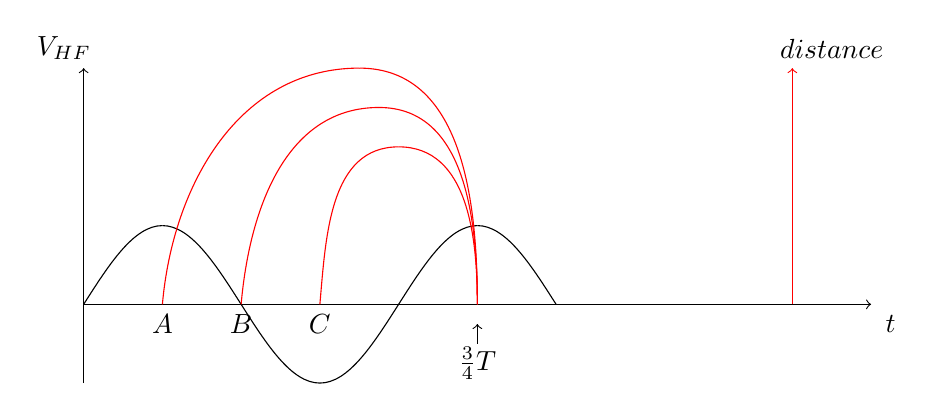
\begin{tikzpicture}
    \draw [->] (0,0) -- (0,4);
    \draw [->] (5,0.5) -- (5,0.75);
    \draw [->] (0,1) -- (10,1);
    \draw [->,red] (9,1) -- (9,4);
    \path node at (-0.25,4.25) {$V_{\text{HF}}$}
          node at (10.25,0.75) {$t$}
          node at (9.5,4.25)  {$\text{distance}$}
          node at (5,0.25) {$\frac{3}{4}T$};
    \draw (0,1) sin (1,2);
    \draw (1,2) cos (2,1);
    \draw (2,1) sin (3,0);
    \draw (3,0) cos (4,1);
    \draw (4,1) sin (5,2);
    \draw (5,2) cos (6,1);
    \path node at (1,0.75) {$A$}
          node at (2,0.75) {$B$}
          node at (3,0.75) {$C$};
    \draw [red] (1,1) to[out=85,in=180] (3.5,4);
    \draw [red] (3.5,4) to[out=0,in=90] (5,1);
    \draw [red] (2,1) to[out=85,in=180] (3.75,3.5);
    \draw [red] (3.75,3.5) to[out=0,in=90] (5,1);
    \draw [red] (3,1) to[out=85,in=180] (4,3);
    \draw [red] (4,3) to[out=0,in=90] (5,1);
  \end{tikzpicture}
  \caption{Darstellung der Geschwindigkeitsmodulation.}
  \label{fig:mod}
\end{figure}

Elektronen, die zu einem früheren Zeitpunkt $A$ in das Hochfrequenzfeld eintreten, werden zusätzlich beschleunigt, wohingegen, welche die zu einem späteren Zeitpunkt $B$ kommen, verlangsamt werden.
Nach passieren des Resonators werden die Elektronen am negativ geladenen Reflektor reflektiert und, bei richtig eingestellter Reflektorspannung, gelangen alle Elektronen zu dem selben Zeitpunkt wieder im Resonator an (bunching), an dem sie maximal abgebremst werden.
Dies findet immer bei $(n+3/4)$ der Periodendauer des Resonators statt.
Die maximale Abbremsung gewährleistet die effektivste Umwandlung in Strahlungsenergie, welche sich im Output wiederspiegelt.\\
Wird die Reflektorspannung nun durchmoduliert, ergibt sich der Zusammenhang von Frequenz und Output, wie er in Abbildung \ref{fig:output} zu sehen ist.

\begin{figure}
  \centering
  \includegraphics[height=6cm]{ressources/output.png}
  \caption{Typisches Signalbild des Versuchs \cite{skript}.}
  \label{fig:output}
\end{figure}

Es sind immer dann Peaks zu sehen, wenn die Reflektorspannung gerade so eingestellt ist, dass ein Elektronenbunch zum Zeitpunkt maximaler Abbremsung in den Resonator zurückkommt.
Ein Peak entspricht dabei einem Modus, welcher durch $(n+3/4)T$, der Aufenthaltsdauer der Elektronen im Resonatorraum, definiert ist.

\subsection{Wellen in einem Hohlleiter}

In dem Hohlleiter breiten sich die vom Klystron erzeugten Mikrowellen aus.
Die elektromagnetische Welle wird an jeder Unstetigkeit bzw nicht charakteristischen Impedanz im Leiter reflektiert.
Bei einer homogenen Leitung unendlicher Ausdehnung, sowie einer Leitung die mit einem Widerstand abgeschlossen ist der die charakteristische Impedanz der Leitung besitzt, treten keine Reflexionen auf.
Im Falle von Reflexionen ergibt sich die Feldstärke durch Addition der Amplituden der einlaufenden und reflektierten Welle, wobei die Amplitude und Phase letzterer von der Amplitude und Phase der reflektierenden Impedanz abhängen.
Durch die Addition bilden sich stehende Wellen im Leiter aus.
Maxima entstehen dort, wo sich die Wellen gleicher Phase addieren, bei Minima haben sie entgegengesetzte Phasen.
Der halbe Abstand zwischen zwei Maxima bzw. Minima definiert die Wellenlänge im Hohlleiter.
Für einen mit Luft gefüllten Hohlleiter gilt für die Wellenlänge
\begin{equation}
  \lambda_\text{g} = \frac{\lambda_0}{\sqrt{1-\left(\frac{\lambda_0}{\lambda_\text{c}}\right)^2}},
\end{equation}
wobei $\lambda_0$ die Wellenlänge im freien Raum und
\begin{equation}
  \lambda_\text{c} = 2a%\frac{2}{\sqrt{\left(\frac{m}{a}\right)^2 + \left(\frac{n}{b}\right)^2}}
\end{equation}
die kritische Wellenlänge für eine Halbwellen-Änderung in eine Richtung eines rechteckigen Hohlleiters mit Breite $a$ ist.
Daher gilt
\begin{equation}
  \lambda_0 = \frac{1}{\sqrt{\left(\frac{1}{\lambda_\text{g}}\right)^2+\left(\frac{1}{2a}\right)^2}} \label{eqn:1}
\end{equation}
und dadurch für die Frequenz
\begin{equation}
  f = \frac{c}{\lambda_0} = c \sqrt{\left(\frac{1}{\lambda_\text{g}}\right)^2+\left(\frac{1}{2a}\right)^2} \label{eqn:2}
\end{equation}
mit der Lichtgeschwindigkeit $c$ im freien Raum.

\subsection{Stehwellenverhältnis}

Das Stehwellenverhältnis bzw die Welligkeit $S$ ist das Verhältnis von maximaler und minimaler Feldstärke im Hohlleiter
\begin{equation}
  S = \frac{E_\text{max}}{E_\text{min}}.
\end{equation}
Es drei verschiedene Methoden die Welligkeit zu messen; die direkte, die "3 db-Methode" und die "Abschwächer-Methode".\\
Bei allen Methoden ist es üblich einen kleinen Teil der Leistung an der Leitung mit einer Sonde abzugreifen.
Das Signal wird an einen Detektor weitergegeben.
Bei der direkten Methode kann die Welligkeit direkt an einem SWR-Meter abgelesen werden.
Diese Methode ist jedoch nur genau bei kleinen Welligkeiten, da bei großen die Sondentiefe erhöht werden muss, was zu Störungen führt.
Die anderen beiden Methoden bieten dabei eine genauere Alternative.\\
Bei der "3 db-Methode" wird der Abstand zwischen zwei Punkten gemessen, an denen die Ausgangsspannung am Detektor den doppelten Wert des Minimums erreicht.
Die Welligkeit ergibt sich dann aus der Formel
\begin{equation}
  S = \sqrt{1+\frac{1}{\sin^2\left(\frac{\pi (d_1-d_2)}{\lambda_\text{g}}\right)}}, \label{eqn:3}
\end{equation}
wobei $d_1$ und $d_2$ die oben beschriebenen Punkte darstellen.\\
Bei der "Abschwächer-Methode" wird das Maximum am Detektor dem Minimum über Einstellen eines Dämpfungsgliedes gleichgemacht.
Dadurch folgt für die Welligkeit die Formel
\begin{equation}
  A_2-A_1 = 20\log(S),
\end{equation}
dabei sind $A_1$ und $A_2$ die Einstellungen des Abschwächers vor und nach der Anpassung.
\cite{skript}

% 2x2 Plot
% \begin{figure*}
%     \centering
%     \begin{subfigure}[b]{0.475\textwidth}
%         \centering
%         \includegraphics[width=\textwidth]{Abbildungen/Schaltung1.pdf}
%         \caption[]%
%         {{\small Schaltung 1.}}
%         \label{fig:Schaltung1}
%     \end{subfigure}
%     \hfill
%     \begin{subfigure}[b]{0.475\textwidth}
%         \centering
%         \includegraphics[width=\textwidth]{Abbildungen/Schaltung2.pdf}
%         \caption[]%
%         {{\small Schaltung 2.}}
%         \label{fig:Schaltung2}
%     \end{subfigure}
%     \vskip\baselineskip
%     \begin{subfigure}[b]{0.475\textwidth}
%         \centering
%         \includegraphics[width=\textwidth]{Abbildungen/Schaltung4.pdf}    % Zahlen vertauscht ... -.-
%         \caption[]%
%         {{\small Schaltung 3.}}
%         \label{fig:Schaltung3}
%     \end{subfigure}
%     \quad
%     \begin{subfigure}[b]{0.475\textwidth}
%         \centering
%         \includegraphics[width=\textwidth]{Abbildungen/Schaltung3.pdf}
%         \caption[]%
%         {{\small Schaltung 4.}}
%         \label{fig:Schaltung4}
%     \end{subfigure}
%     \caption[]
%     {Ersatzschaltbilder der verschiedenen Teilaufgaben.}
%     \label{fig:Schaltungen}
% \end{figure*}
